\section{Defining and Applying the SEA Technique}
\label{SEC:approach}

\begin{figure}[t]
  \center{}
  \fbox{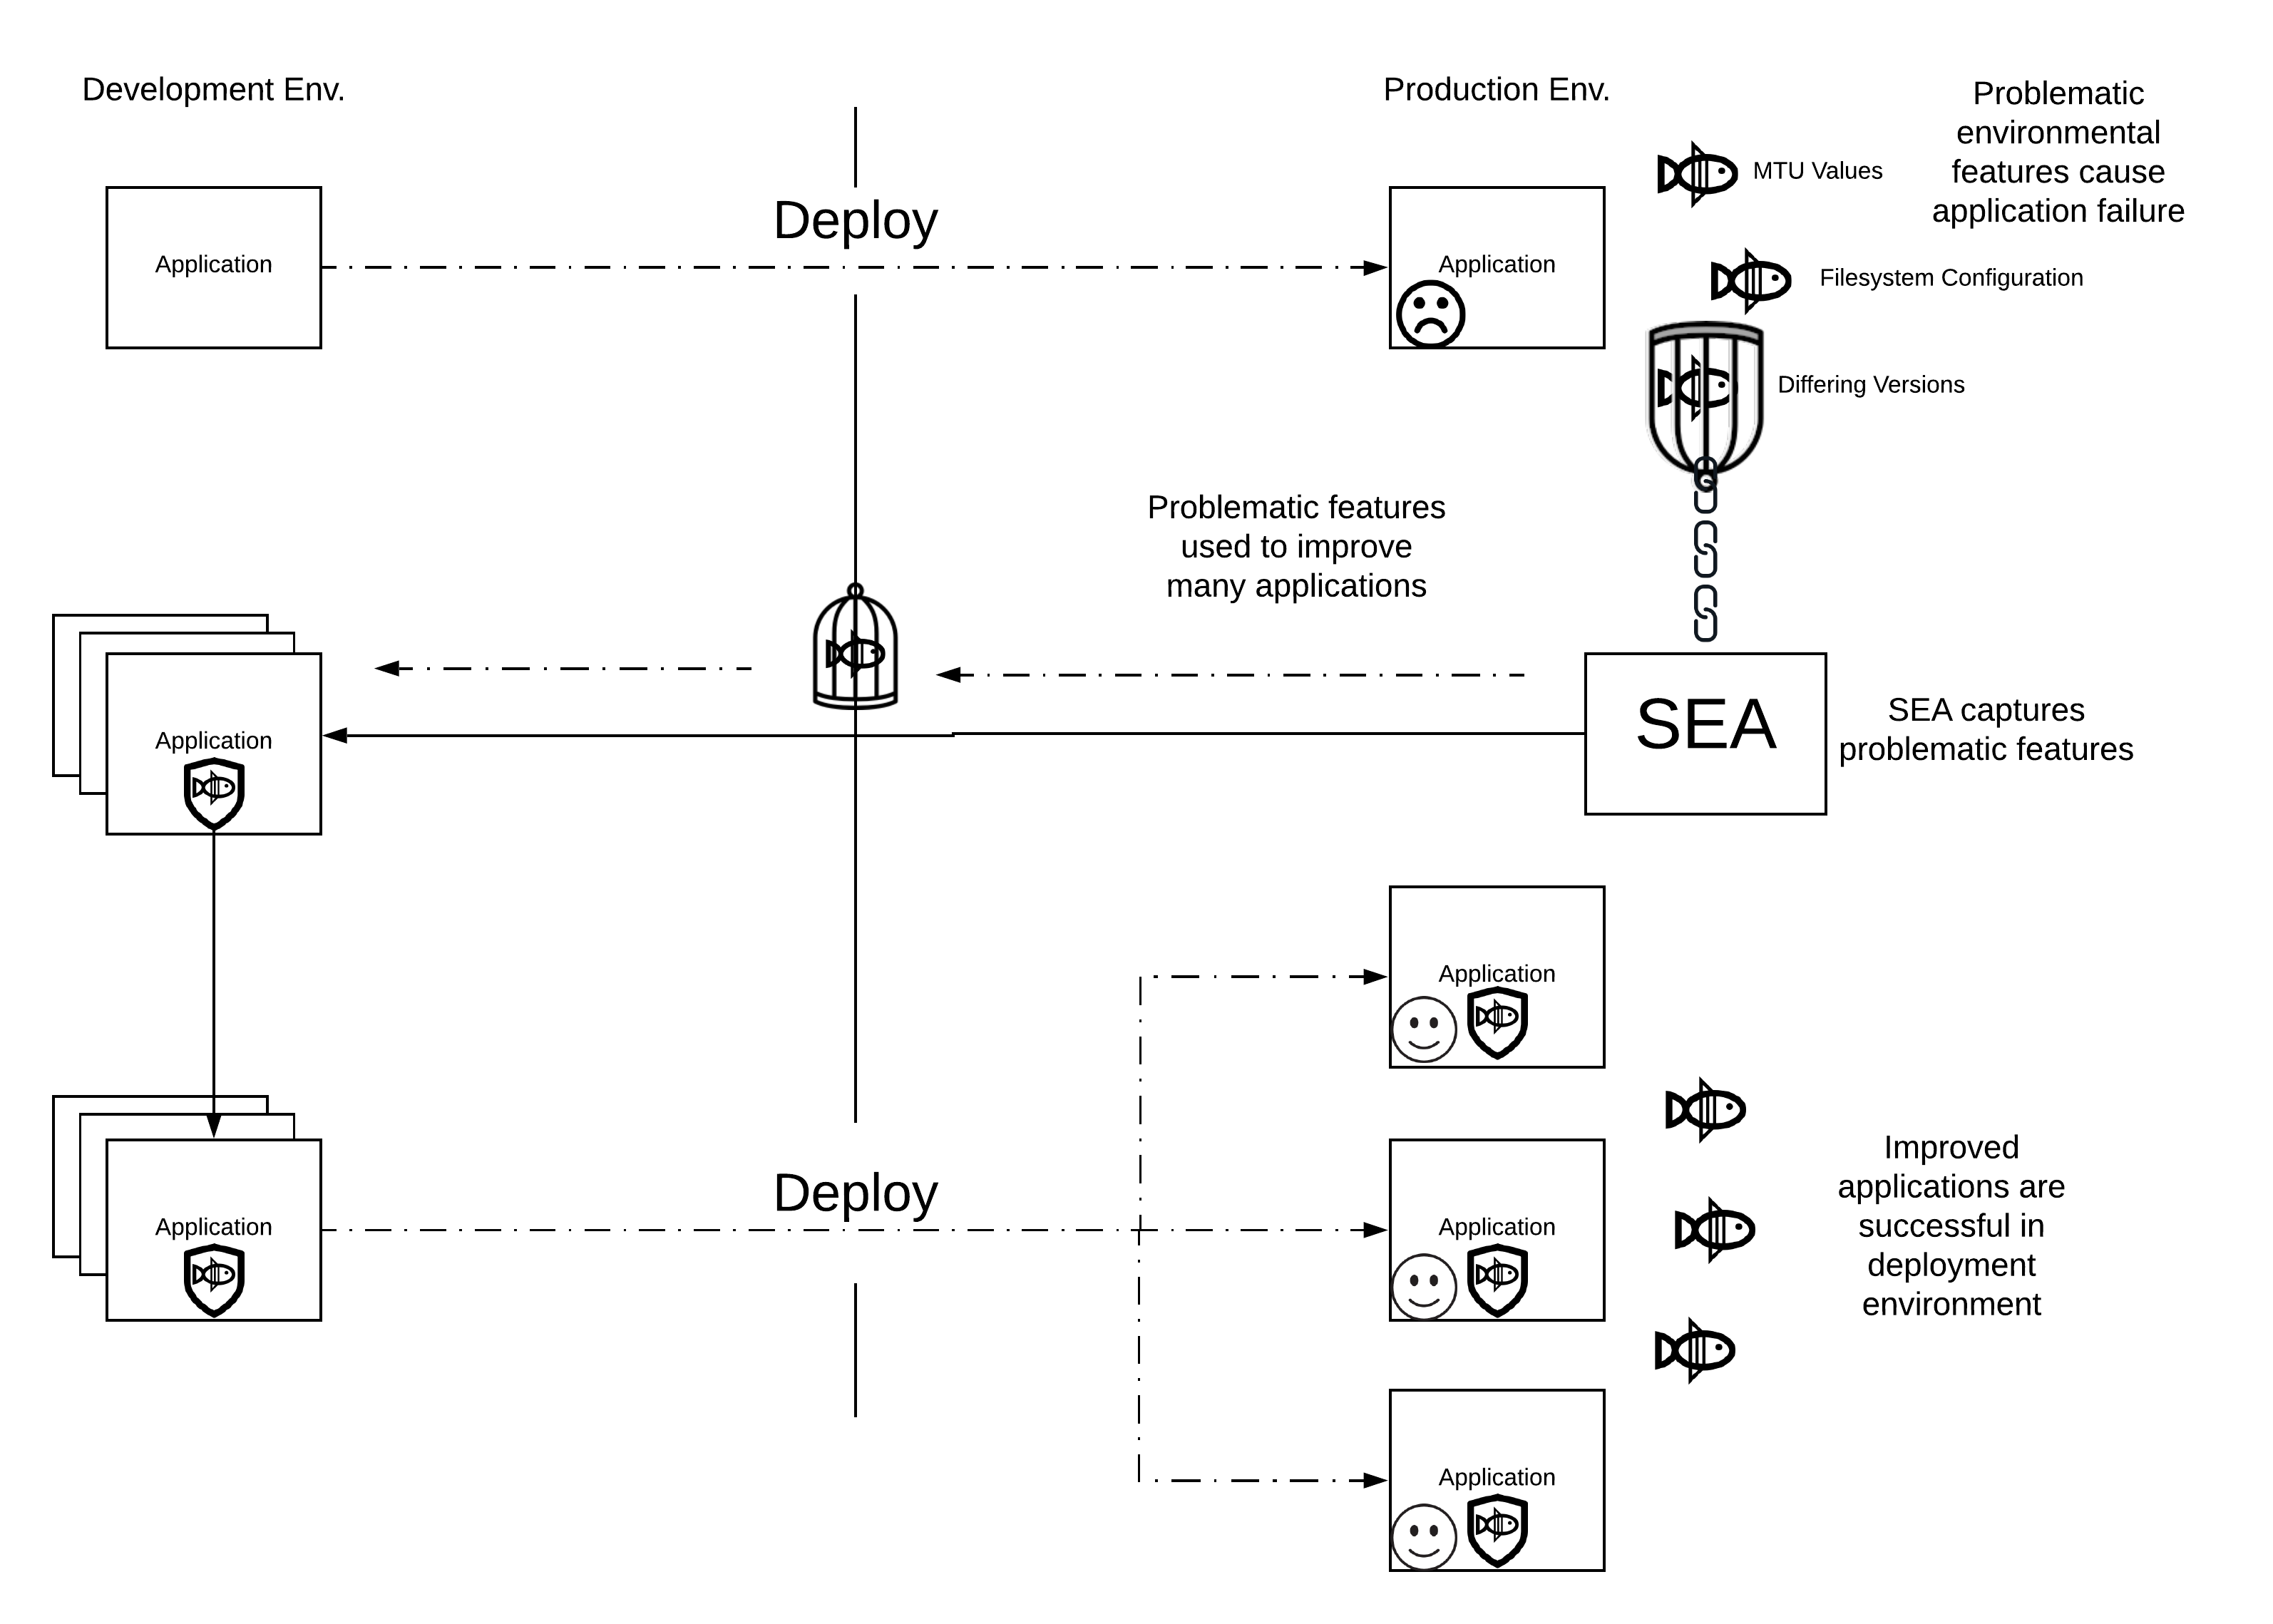
\includegraphics[scale=.37]{images/approach}}
  \caption{Using SEA allows developers to capture features that make an
    environment problematic and use them to prevent future applications
    from falling victim to the bugs of the past.}
  \label{figure:approach}
\end{figure}

\begin{figure*}[t]
  \center{}
  \fbox{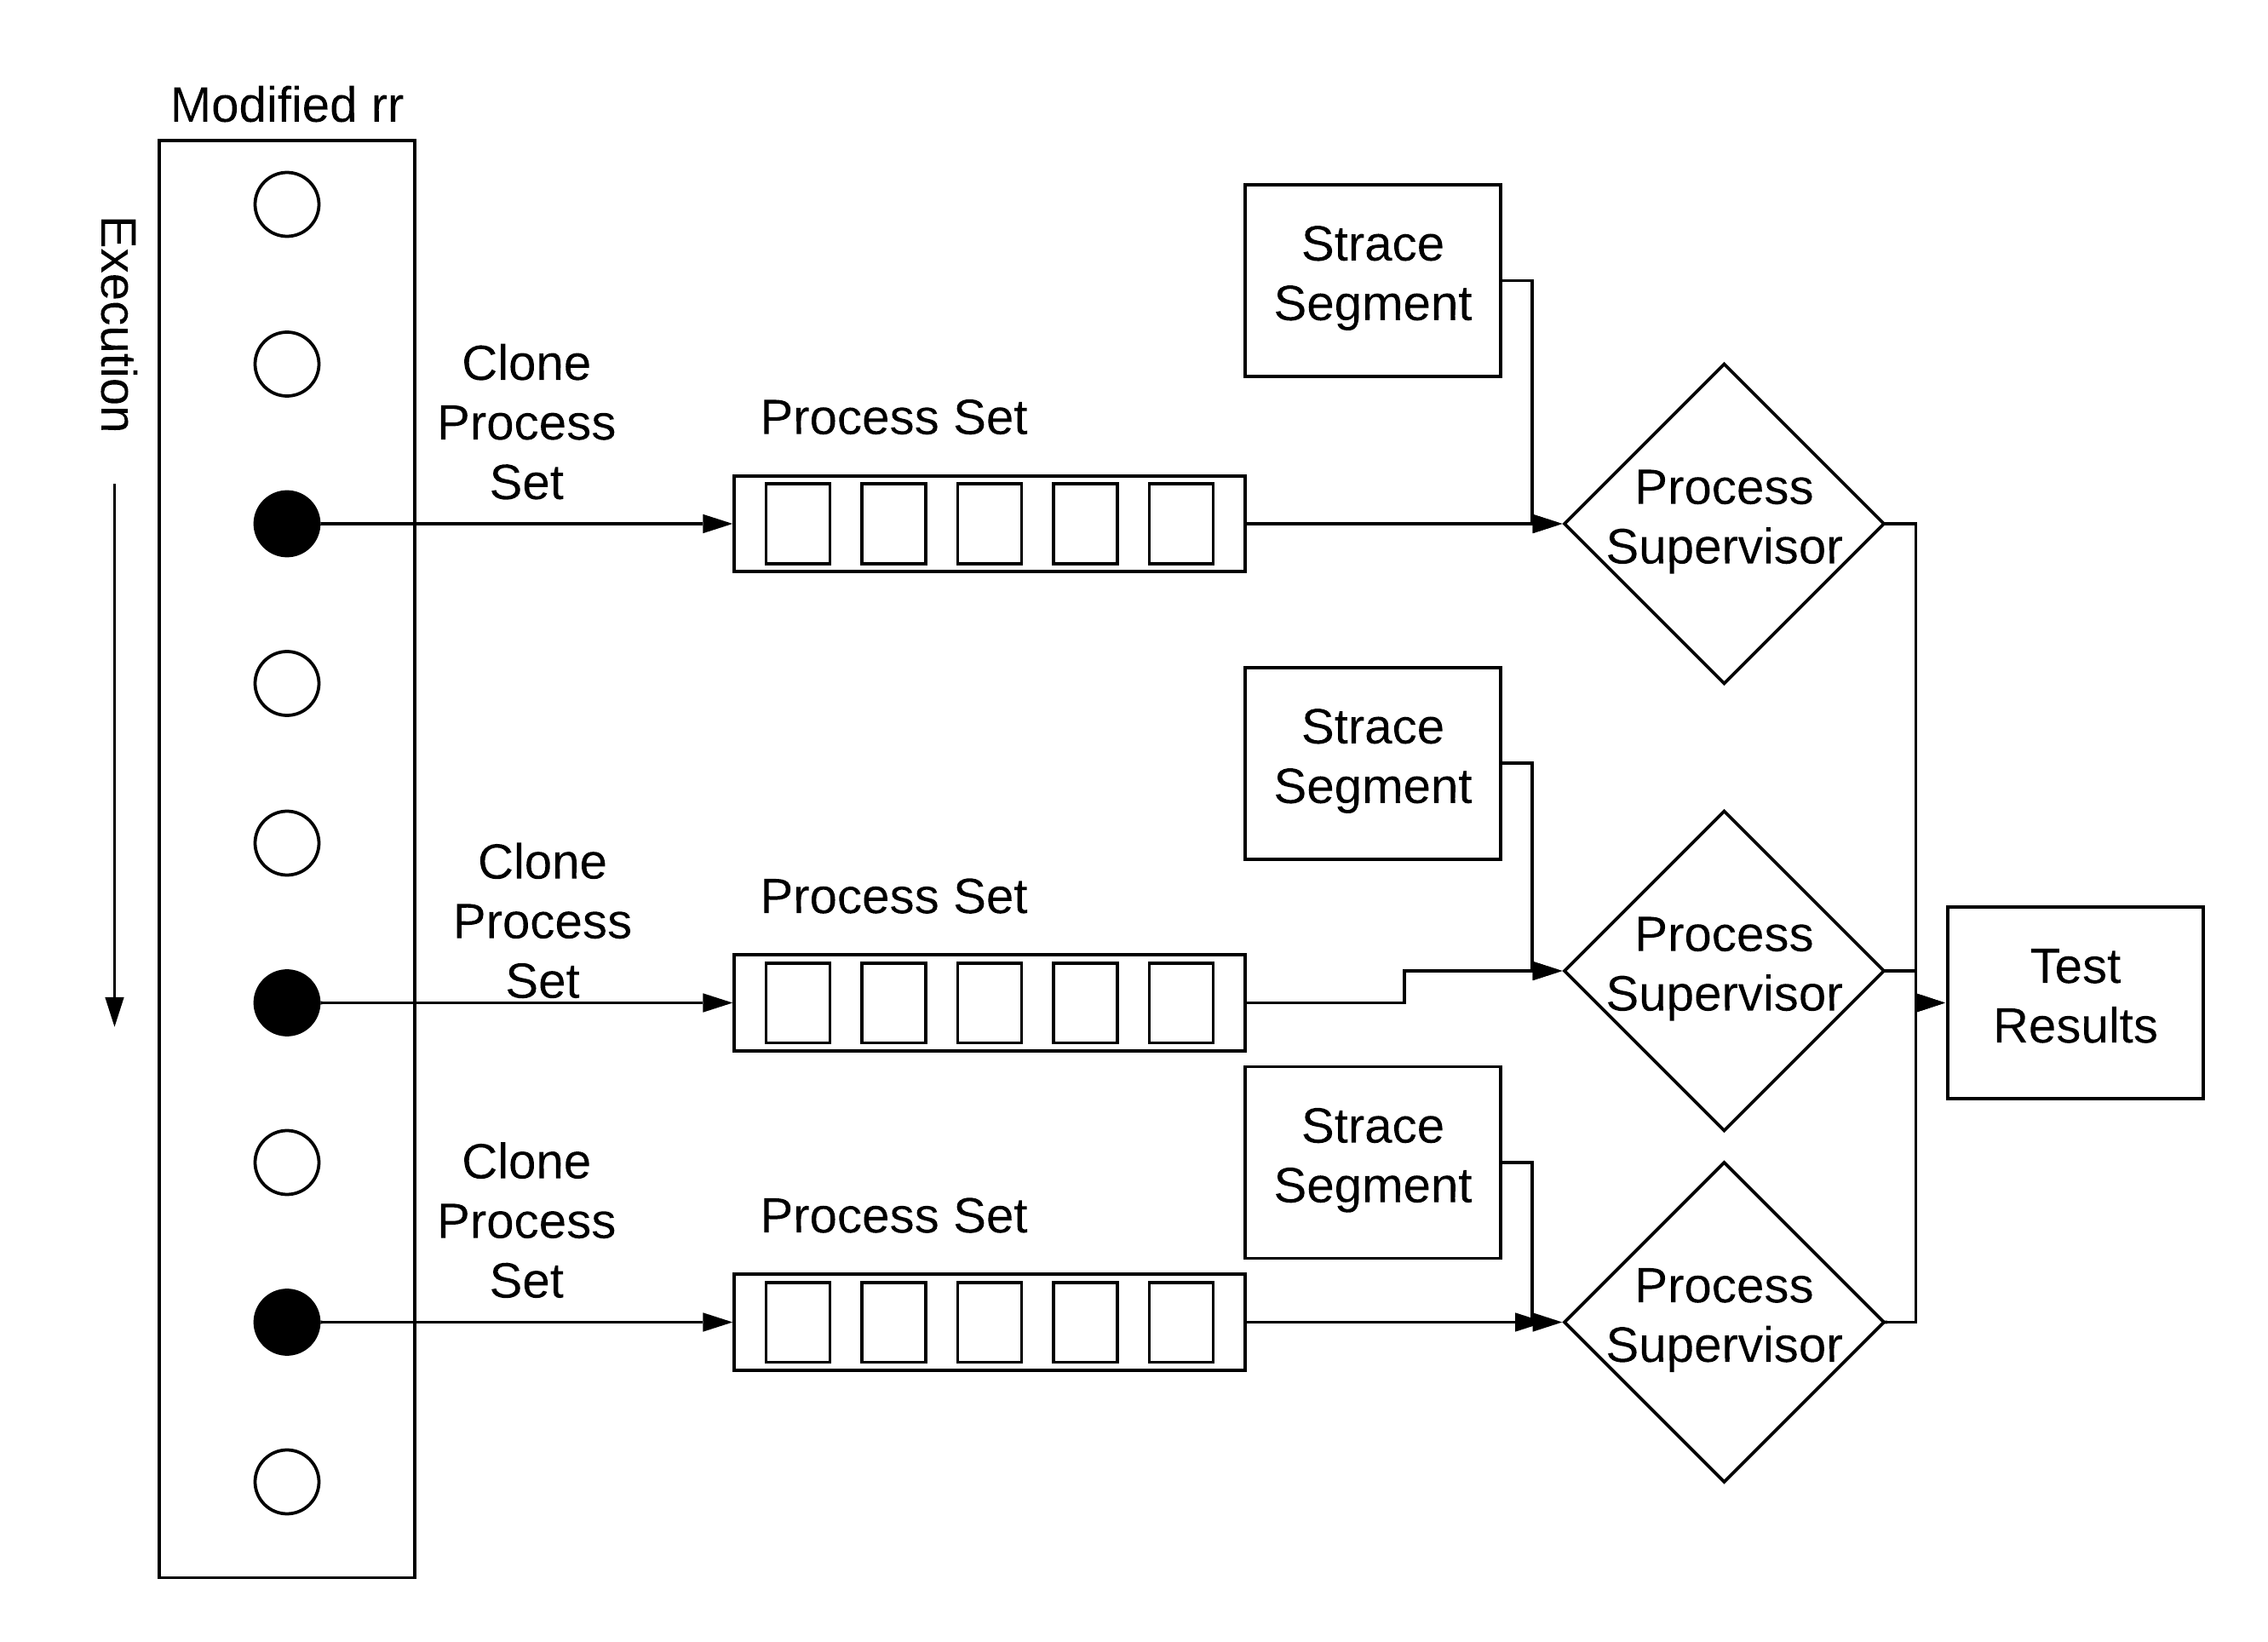
\includegraphics[scale=.65]{images/architecture}}
  \caption{Diagram illustrating CrashSimulator's Architecture.  During the
    course of a single rr execution, clone process sets are generated at
    specific rr events.  A CrashSimlator supervisor process attaches to
    these process sets and uses a strace-style system call listing to feed
    subsequent system call activity and inject unusual environmental
    conditions.}
  \label{figure:architecture}
\end{figure*}

As mentioned earlier,
the Simulation of Anomalous Environments (SEA)
offers a reliable way to identify bugs that could arise from interaction
with a given environment.
It does this by providing a systematic way of
capturing, storing and utilizing the insights gleaned from the work that
went into debugging previous failures in a given environment.
In this section, we offer a high-level look at how SEA works, followedb by
a more in-depth look at tits primary operations.
Finally, we detail our concrete implementation, CrashSimulator.

\subsection{SEA in a Nutshell}
\label{SEC:SEANutshell}
In a nutshell,
here is how the technique works.
An application is run
in a particular environment and fails.
In debugging the failure,
we identify and ``trap'' the particular environmental feature
(sec.~\ref{SUBSUB:IdentifyingAndEncoding}),
that caused the crash,  which we call $X$.
We verify that when $X$ is present,
communication with the
environment is different,
sometimes in a barely perceptible manner,
and other times in a radically contrary manner.
We call this difference $X'$.
$X'$ can be extracted, preserved,
and later used in testing other systems
thanks to a pair of components referred to as a mutator and a checker.
The mutator describes the exact set of changes
that must be made to an application's communications
in order to simulate an anomaly,
while the checker describes how an
application should respond once the anomaly has been encountered.
To test if other applications also have a problem with $X$,
mutators can insert $X'$ into their
communications (sec.~\ref{SUBSUB:MutatingCommunications}).
A checker will then determine whether the
application has responded correctly to
$X$(sec.~\ref{SUBSUB:CheckingResponse}).
If the checker accepts the application behavior
after the anomaly is simulated,
we report it has been handled.
If the checker doesn't accept we report that it hasn't.
Once created,
these pieces act as the persistent medium in which the details of
a given anomaly are stored.

Preserving this information in an accessible manner
is a boon for software developers because,
in a typical scenario, the material documenting
the discovery of flaws
either goes out of date or
is preserved only as ``institutional memory,''
and therefore forgotten as staffs change.
Additionally,
the mere existence of documentation
describing past failures
does not prevent bugs
if developers don't use it
to construct and execute tests,
an effort that is easily neglected.
Further, unit and integration test suites
are typically tightly coupled
to the application and the programming language in which it was written --
limiting their reusability.
SEA cuts through all of these difficulties by
storing this information in a manner that can be consumed
and used to test applications programmatically.
In this section, we discuss each of the components
required to implement SEA
and detail our concrete implementation,
CrashSimulator~\ref{SUBSEC:ApproachCrashSim}.

\section{Primary Operations}
\label{SEC:PrimaryOperations}

To take a closer look at how SEA functions,
we divide the technique
into its three primary operations.
These are:
identifying and trapping anomalies,
mutating application communications,
and checking application responses.

\subsubsection{Identifying and Encoding Anomalies}
\label{SUBSUB:IdentifyingAndEncoding}
At the core of SEA's operation is the body of anomalies
used to test applications.
Building this corpus is an ongoing process that improves the technique's
effectiveness by extending the set of environments it can simulate.
Anomalies can be sourced
in a number of ways,
such as
examining the failures of other applications
in a target deployment environment,
or by using other tools that can identify
potentially problematic behavior in other domains~\cite{Zhuang_NSDI_2014,
rasley2015detecting}.
Public bug trackers are an ideal source
if you wish to determine
whether or not an application
is vulnerable to a widely publicized bug.
The chosen anomalies are then examined
to determine how they change an application's communications
with its environment
compared to a normal execution and why.
Once teased out,
these differences delineate
a set of modifications
that must be made to an application's communications
in order to simulate the chosen anomaly or anomalies.
The details of the anomaly are used to
construct both a mutator,
which contains the modifications in question,
and a checker
(or set of checkers)
which encodes how the application should respond to that modification.
Describing anomalies in this fashion
allows them to be recorded systematically and cataloged for future use.

Consider,
for example,
an anomalous environment
where access to a required file is denied because of
the environment's file security configuration.
With this anomaly,
attempts to access the file
such as calls to {\tt fread()},
or the {\tt read()} system call,
will fail with an error stating that access to the file is denied.
The ``modification'' required to simulate this anomaly
is to change the results of similar accesses
in a test execution
to return ``access denied.''
This anomaly can be preserved by constructing a mutator that describes how
a failing {\tt read()} call differs from a normal one and a checker that checks for
the application altering its behavior in response.

\subsubsection{Mutating Communications}
\label{SUBSUB:MutatingCommunications}
Simulating an environmental anomaly requires specific interventions at the
correct moments during an execution.
As a result,
SEA requires
an application's communications
with its environment
be monitored
by such means as
redirecting function calls,
observing memory access,
monitoring network activity,
or intercepting system calls.
Looking at the parameters,
return values,
and orderings
of an application's communications
can indicate
when would be an appropriate time to simulate an anomaly.

Once an opportune moment has arisen,
the technique requires that its implementer
interpose on the application's communications
and make the modifications necessary
to simulate the presence
of the anomaly.
This could be accomplished
a number of ways,
such as
by influencing the results of function calls or system calls,
or strategically altering memory values.
In the simplest case,
simulating an anomaly only requires
the modification of a single value.
In more complex cases,
large numbers of diverse communications
need to be interdicted and altered
in order to correctly simulate an anomaly.
For example,
simulating an erratic system clock
requires that all efforts
to access the clock
be modified to reflect the chosen aberration.

\subsubsection{Checking an Application's Response}
\label{SUBSUB:CheckingResponse}
SEA relies on checkers
to provide a flexible approach to assess the way an application
behaves after it has encountered an anomaly.
A checker is constructed to store
some behavior that the application should undertake
in response to the anomaly being simulated.
It looks for this behavior by examining an application's communications
before, during, and after the simulation of an anomaly.
The checker then reports whether the application has handled
the anomaly based on whether or not it observed the behavior for which it
was built to look.

As an example, consider the ``default checker'' from CrashSimulator.
It draws a conclusion based on
whether or not the application
has made an effort to respond
to the anomaly.
This determination is made based
on the assumption
that such a response will yield
different program paths (and therefore different communications).
If the application
does not alter its behavior, it has not
correctly handled this flaw.
Alternatively,
if the application does deviate,
it is likely
an action has occurred to handle the simulated condition.
This simple yes or no approach
is often sufficient
to classify application behavior.



\subsection{CrashSimulator: A Concrete SEA Implementation}
\label{SUBSEC:ApproachCrashSim}
Evaluating SEA in a real-world fashion requires a
concrete implementation of its components.
We built this implementation into a tool we call CrashSimulator.  The
prototype was built on rr version 5.2.0 running on a 32-bit Linux kernel
distributed with Ubuntu 16.04 LTS.  The modifications to rr, which are
explained in this section, were carried out in C++ and the CrashSimulator
supervisor was implemented in ZZZZ lines of Python 2.7 code with a YYYY
line C extension that allows it to interact with processes using the Ptrace
API.
This version of CrashSimulator is available as a Docker container and,
due to some operating system configuration being necessary, is most easily
installed in this fashion.

Below, we explain CrashSimulator, highlighting a
few central principles that guided our design decisions. The first such
decision was to operate at the system call level, rather than manipulating
calls to library functions, memory accesses, or other points where we could
influence an application's communications. Making this choice provided us a
few key advantages. First, there is already robust tooling in the Linux
kernel that allows for the interception and modification of system call
results and side effects. Additionally, Linux system call semantics are
well defined which simplifies implementation. Finally, operating at this
level allows CrashSimulator to test applications written in any language
that can execute Linux system calls.

Our first task was
gathering a corpus of anomalies to test applications
against.  These anomalies (which are discussed
in Section~\ref{SEC:evaluation})
were collected by examining public bug trackers,
the source code of major portable applications, and the capabilities of
tools like NetCheck~\cite{Zhuang_NSDI_2014}
and CheckAPI~\cite{rasley2015detecting}.
From these anomalies,
we constructed
checkers and mutators
using finite automata.
Mutators work by receiving the sequence of system calls
an application makes and accepting situations where the sequence indicates
it is appropriate to simulate an anomaly.
It then uses its stored
description of an anomaly
to carry out its simulation.
Checkers operate similarly,
but, because they encode what a
correct response by the application should look like,
they were constructed
to accept situations where they observed sequences indicative of such
behavior.
%This process required manual effort and expertise.
%However,
%much like
%the effort involved in constructing a unit test to check for correct
%behavior in a piece of code, we found that this initial outlay of
%user skill and effort was paid back, as
%we were able to use its products
%repeatedly over time to test many different applications.

CrashSimulator monitors an application by
recording it
using a modified version of the {\tt rr}!!CITE!!
debugger.
The modifications allow
a {\tt strace}-style
system call recording to be output alongside {\tt rr's} normal recording
format, providing
a complete log of an applications system call activity. Mutators and
checkers operate on this log to find opportunities to simulate
anomalies and evaluate an application's response.

Actually simulating anomalies
is done using
a technique
we call {\it process set cloning}.
The {\tt rr} debugger manages,
and can copy,
the full set of processes underlying an application
so that users can test debugging
hypotheses without damaging the original.
We extended this capability
by liberating process set copies from {\tt rr}.
This means that given application $Y$
consisting of processes $a$, $b$, and $c$
(written as $Y(a, b, c)$),
we can generate cloned sets $Y_1(a_1, b_1, c_1)$,
$Y_2(a_2, b_2, c_2)$ ... $Y_n(a_n, b_b, c_n)$.
$Y_1$, $Y_2$ ... $Y_n$ can then be used to test different scenarios leaving
the original $Y$ to continue its execution unhindered.
Process sets generated in this fashion are created in a stopped state and
remain that way until they are attached to and utilized by a CrashSimulator
supervisor.

Once a supervisor has attached to a process set, it uses the above {\tt
strace} log and the output of a mutator to service any future
system calls the application makes.  In this way, the mutator is able to
influence system call results and simulate its anomaly.
During this process,
a corresponding checker
monitors the application's behavior allow it to report on its correctness.
This allows testing in the following way.
At a given point in execution of application $Y$,
$Y_1$ and $Y_2$ are generated and
used to test two scenarios where a file access fails:
\begin{enumerate}
    \item{For $Y_1$, access to the file is denied due to a permissions issue}
    \item{For $Y_2$, access fails because of an I/O error}
\end{enumerate}
The simulations for both $Y_1$ and $Y_2$ are handled asynchronously and
the results reported.
This approach allows many tests to be run independently of one another,
which lends a
high degree of speed and
parallelism to the testing process.
At the same time, the original $Y$ execution continues unhindered to the
next simulation opportunity where this process repeats.
Keeping $Y$ intact
(as opposed to destroying it by introducing an error state)
avoids the penalty
of having to restart a new execution for each test.
